\subsection{Použitie hybridných modelov}
V predchádzajúcich častiach sme ukázali ako si s problematikou optimalizácie prevádzky zariadenia, pri nepresnom matematickom opise, dokázali poradiť dvojkroková optimalizácia a schéma úpravy modifikátora. Poďme sa pozrieť ako sa s touto problematikou dokáže vysporiadať prístup s použitím hybridných modelov.

V časti \aps{trénovanie dátových modelov} sme identifikovali dva typy FIR modelov -- jeden na údajoch rozdielov koncentrácie biomasy a druhý na dátach substrátu. Tieto modely využijeme na úpravu ustálených stavov nepresného mechanického modelu, pomocou ktorého sa snažíme docieliť optimálnu prevádzku zariadenia. Demonštrujme si najskôr výsledky optimalizácie hybridného modelu odvodeného na dátach biomasy.

Výsledky priebehu optimalizácie sú zobrazené na Obr. \ref{fig:hybrid_bio_opt_results}. Ako si môžeme všimnúť na Obr. \ref{fig:hybrid_bio_costFun}, kde sú znázornené optimá hybridného modelu vyjadrené ako hodnoty účelovej funkcie zariadenia v jednotlivých iteráciách, tak takýto prístup dostane naše zariadenie v troch krokoch do optimálneho stavu, ktorý je zobrazený bodkovanou čiarou. V neskorších iteráciách sa mení optimum hybridného modelu a ustálený stav nášho zariadenia sa vzďaľuje od svojho optimálneho ustáleného stavu. Tento jav je spôsobený tým, že šum merania je omnoho výraznejší ako samotná skoková zmena a preto aj predikovaný ustálený stav nebude tak presný. To môžeme vidieť na Obr. \ref{fig:hybrid_bio_ss}, kde v tretej iterácii bol odhadnutý ustálený stav vysoko nadhodnotený. V každej ďalšej iterácií, odhadnutá rýchlosť riedenia $ D $ už neprinesie výraznú skokovú zmenu vzhľadom na šum merania, čím sa znižuje aj informačná výdatnosť dát a hodnota predikovaného ustáleného stavu nám klesá. Fakt, že od tretej iterácie nie sú naše dáta informačne výdatné, môžeme sledovať na Obr. \ref{fig:hybrid_bio_order}, kde je zobrazený rád FIR modelu v jednotlivých iteráciách, ktorý sa od tretej iterácie nemení. V opačnom prípade, by so zvyšujúcim sa počtom dát musel rásť aj rád modelu, kvôli nelinearite nášho zariadenia.
\begin{figure}
	\centering
	\begin{subfigure}[b]{0.49\textwidth}
		\centering
		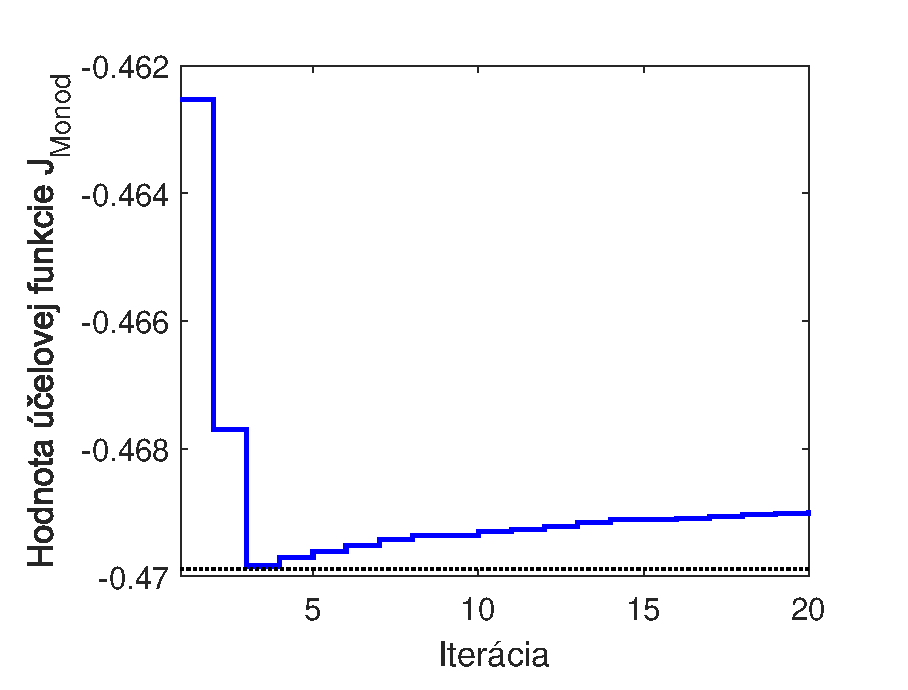
\includegraphics[width=\linewidth]{images/hybrid_bio_costFun}
		\caption{Optimá hybridného modelu vyjadrené ako hodnota účelovej funkcie Monod modelu (zariadenia).}
		\label{fig:hybrid_bio_costFun}
	\end{subfigure}
	\hfill
	\begin{subfigure}[b]{0.49\textwidth}
		\centering
		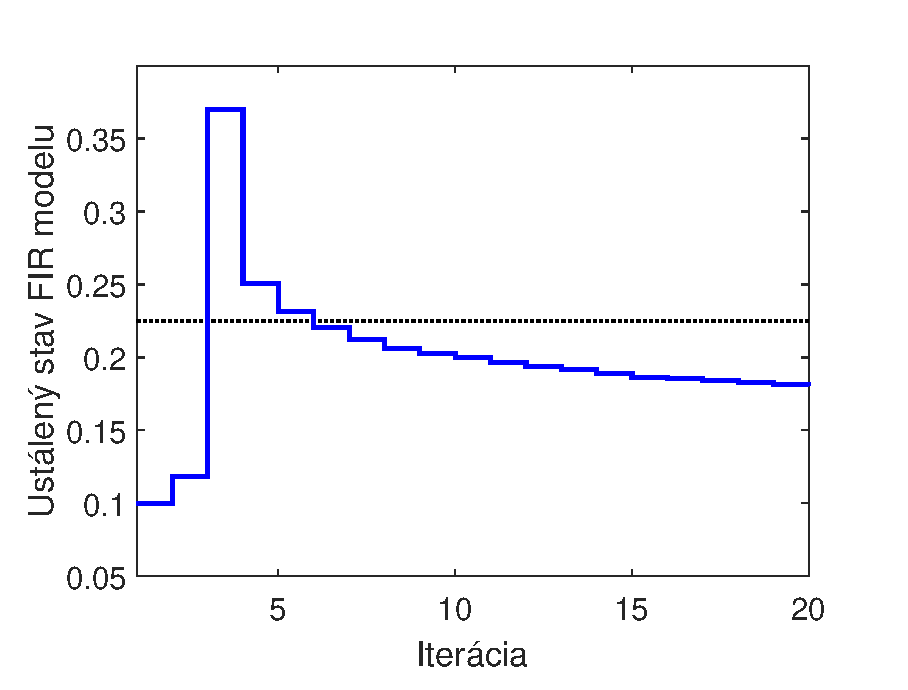
\includegraphics[width=\linewidth]{images/hybrid_bio_ss}
		\caption{Priebeh predikcie ustáleného stavu FIR modelom. \newline}
		\label{fig:hybrid_bio_ss}
	\end{subfigure}
	\bigskip
	\begin{subfigure}[b]{0.49\textwidth}
		\centering
		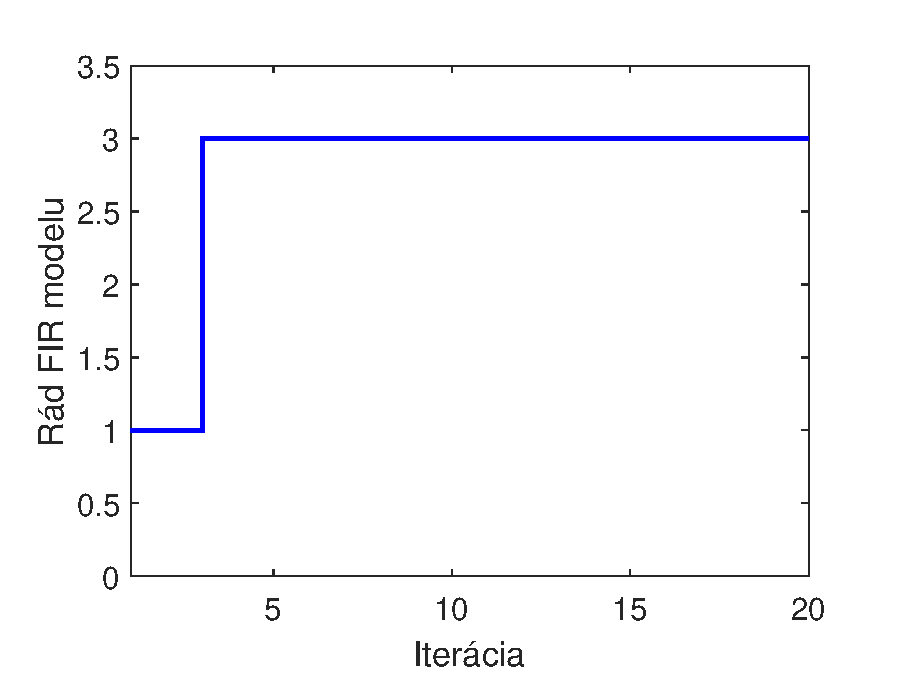
\includegraphics[width=\linewidth]{images/hybrid_bio_order}
		\caption{Priebeh rádu FIR modelu.}
		\label{fig:hybrid_bio_order}
	\end{subfigure}
	\caption{Výsledok optimalizácie pomocou hybridného modelu, identifikovaného na dátach rozdielov koncentrácie biomasy medzi zariadením a nepresným mechanickým modelom.}
	\label{fig:hybrid_bio_opt_results}	
\end{figure}

V skutočnosti, by sme takýto hybridný model mohli len veľmi ťažko skonštruovať. Fluktuácia koncentrácie biomasy, ktorú by sme namerali v biochemickom reaktore, by bola omnoho väčšia ako uvažujeme my ($ W_{x} = 0.05\si{\gram\per\liter} $). To by viedlo k ešte väčšej nepresnosti predikcie rozdielov ustálených stavov koncentrácie a pri optimalizácii by sme mohli získať také rýchlosti riedenia $ D $, ktoré by dostali naše zariadenia do stavu vymytia. A tak isto, množstvo nameraných údajov by bolo výrazne menšie. Preto si teraz ukážeme výsledky optimalizácie hybridným modelom, odvodeného na dátach koncentrácie substrátu. 

Ako môžeme vidieť na Obr. \ref{fig:hybrid_sub_costFun}, tak takýto hybridný model dokáže skonvergovať do blízkosti optima zariadenia, nie však úplne k nemu. Ale na rozdiel od  predchádzajúceho hybridného modelu, po dosiahnutí maxima sa už z neho nepohne a táto stabilita je veľmi dobrá vlastnosť, pretože zaručuje aspoň nejaký výsledok. V ďalších iteráciách, získaná rýchlosť riedenia $ D $ už nedokáže vyprodukovať skokovú zmenu, ktorá by výrazne zmenila štruktúru dátového modelu a preto sa dostaneme do ustáleného režimu. Toto potvrdzujú aj Obr. \ref{fig:hybrid_sub_ss} a \ref{fig:hybrid_sub_order}, ktoré zobrazujú predikciu ustáleného stavu FIR modelom a jeho rád v jednotlivých krokoch optimalizácie.
\begin{figure}
	\centering
	\begin{subfigure}[b]{0.49\textwidth}
		\centering
		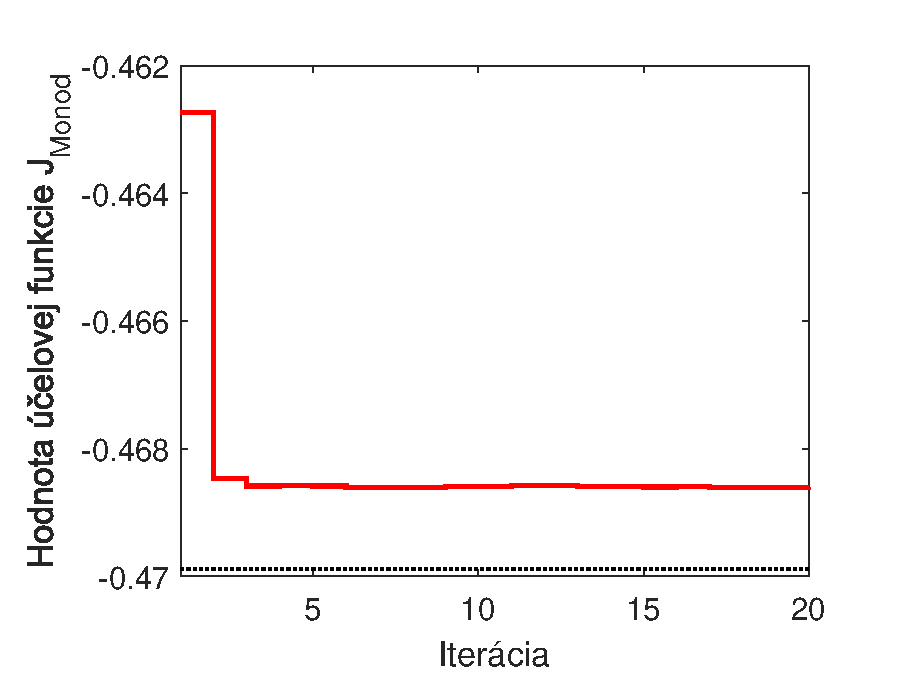
\includegraphics[width=\linewidth]{images/hybrid_sub_costFun}
		\caption{Optimá hybridného modelu vyjadrené ako hodnota účelovej funkcie Monod modelu (zariadenia).}
		\label{fig:hybrid_sub_costFun}
	\end{subfigure}
	\hfill
	\begin{subfigure}[b]{0.49\textwidth}
		\centering
		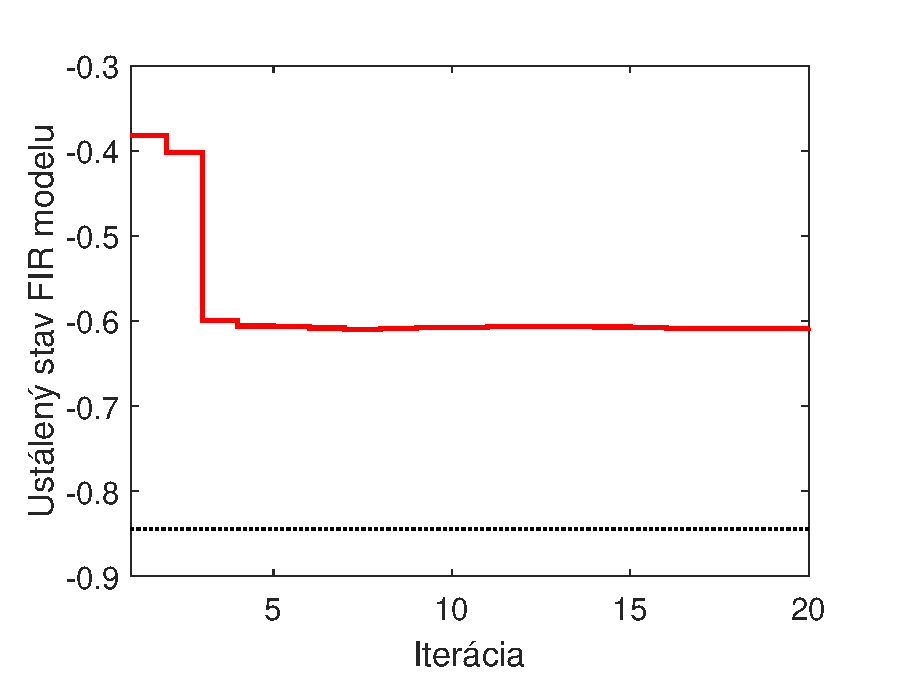
\includegraphics[width=\linewidth]{images/hybrid_sub_ss}
		\caption{Priebeh predikcie ustáleného stavu FIR modelom. \newline}
		\label{fig:hybrid_sub_ss}
	\end{subfigure}
	\bigskip
	\begin{subfigure}[b]{0.49\textwidth}
		\centering
		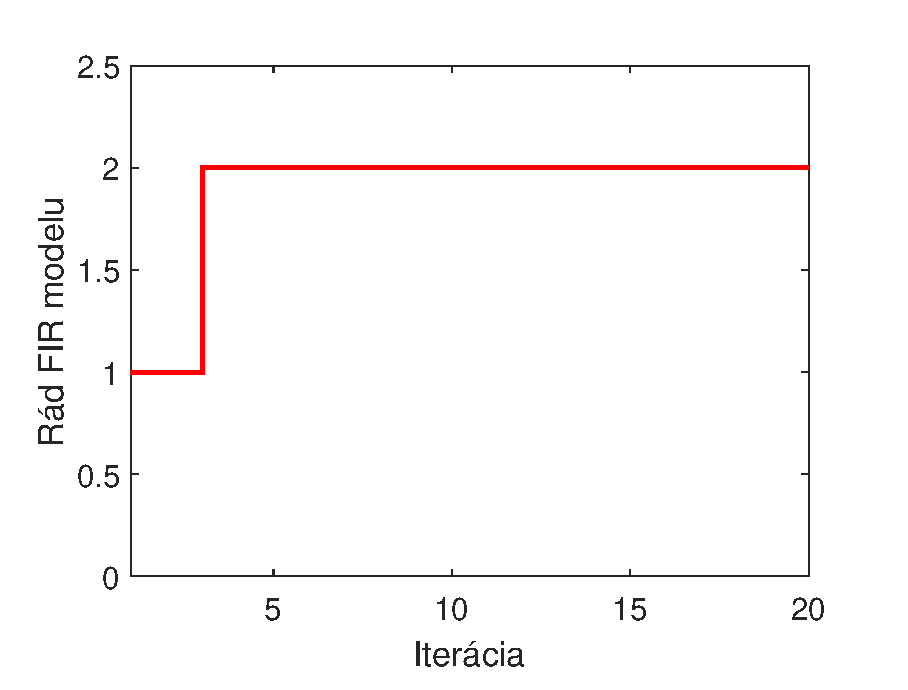
\includegraphics[width=\linewidth]{images/hybrid_sub_order}
		\caption{Priebeh rádu FIR modelu.}
		\label{fig:hybrid_sub_order}
	\end{subfigure}
	\caption{Výsledok optimalizácie pomocou hybridného modelu, identifikovaného na dátach rozdielov koncentrácie substrátu medzi zariadením a nepresným mechanickým modelom.}
	\label{fig:hybrid_sub_opt_results}	
\end{figure}

Na tomto mieste by sme si mohli položiť otázku \aps{Ktorý z hybridných modelov je lepší ?}. Kvôli vplyvu šumu sa hybridný model, založený na korekcii koncentrácie biomasy, dostal výrazne bližšie k optimu zariadenia. Na druhej strane, hybridný model, založený na korekcii koncentrácie substrátu, nám dokáže zaručiť stabilnú rýchlosť riedenia $ D $, ktorá je v relatívnej blízkosti od optima zariadenia. Aby sme mohli tieto dva hybridné modely porovnať, zhotovili sme experiment, v ktorom sme zmenili rozptyl šumu merania koncentrácie biomasy ($ W_{x} = 0.001\si{\gram\per\liter} $) tak, aby bol porovnateľný s rozptylom šumu merania koncentrácie substrátu, vzhľadom na skokové zmeny generované v jednotlivých iteráciách. Výsledok tohto experimentu nám ukázal, že oba hybridné modelu konvergujú k rovnakým hodnotám, ako môžeme vidieť na Obr. \ref{fig:hybrid_sub_and_bio_compar}, ale hybridnému modelu, založenom na úprave koncentrácie biomasy, to trvá o niekoľko iterácií dlhšie. Je to spôsobené najmä tým, že dynamika priebehu koncentrácie biomasy nie je tak výrazná ako priebeh koncentrácie substrátu. Ako sme už vyššie uviedli, tak s touto veličinou je spojených viacero problémov a z tohto dôvodu budeme ďalšie výsledky vzťahovať výlučne na hybridný model substrátu. 
\begin{figure}
	\centering
	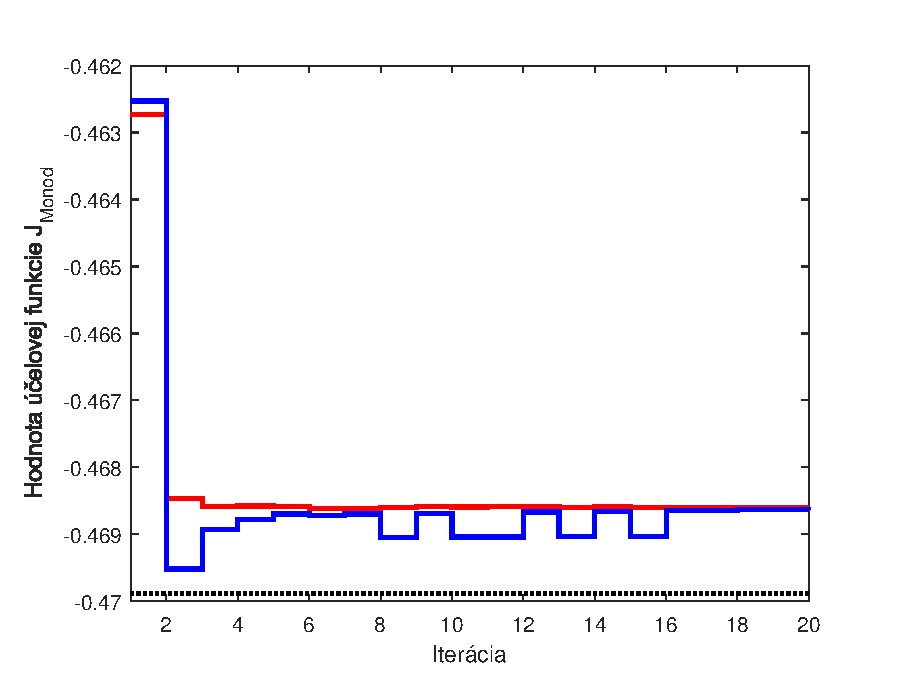
\includegraphics[width=0.7\linewidth]{images/hybrid_sub_and_bio_compar}
	\caption{Porovnanie výsledkov optimalizácie hybridných modelov biomasy a substrátu, vyjadrených ako hodnoty účelovej funkcie Monod modelu (zariadenia). Bodkovanou čiarou je zobrazená skutočná hodnota ustáleného stavu zariadenia.}
	\label{fig:hybrid_sub_and_bio_compar}
\end{figure}

Zistili sme, že iteračným prístupom sa dokážeme dostať iba do blízkeho okolia optimálneho ustáleného stavu zariadenia, nedokážeme však odhadnúť samotné optimum. Preto si dovolíme tvrdiť, že iteračný prístup v spojení s hybridným modelovaním nie je najlepšou voľbou optimalizácie prevádzky zariadenia. Ale k optimalizácii pomocou hybridných modelov môžeme pristupovať ešte iným spôsobom. Dátové časti hybridných modelov majú veľkú výhodu a tou je, že ich môžeme natrénovať na historických údajoch dopredu. Takto už bude mať dátový model nejaké informácie o systéme v sebe uchované. Limitovaný sme iba množstvom dát, ktorým disponujeme a od toho závisí kvalita predikcie modelu. 

Predstavme si situáciu, že máme k dispozícii namerané údaje rozdielu koncentrácie substrátu. Tie zodpovedajú piatim skokovým zmenám v rýchlosti riedenia $ D = \lbrace 0.3760, 0.3845, 0.3930, 0.4015, 0.4100 \rbrace \si{\per\hour} $, kde najnižšia hodnota predstavuje optimálnu rýchlosť riedenia nominálneho modelu $ D_{N}^{\star} $. Na týchto dátach sme identifikovali pomocou garantovaného odhadu parametrov FIR model. Aby sme sa vyhli modelom zbytočne vysokého rádu, museli sme zmeniť chybu modelu $ \delta_{s} $ na osemnásobok rozptylu šumu merania $ \delta_{s} = 0.2\si{\gram\per\liter} $. Takto sme získali FIR model 6. rádu a jeho výstup môžeme vidieť na Obr. \ref{fig:hybrid_multipleStep_data}. Určite sa zhodneme, že takýto FIR model nemá veľa spoločného s realitou, ale ide o krásnu ukážku aproximácie nelineárneho systému lineárnym dátovým modelom. Keď sme takýto model použili na korekciu ustálených stavov koncentrácie substrátu nominálneho modelu pri optimalizácii, získaná rýchlosť riedenia $ D $ uviedla naše zariadenie do jeho optimálneho ustáleného stavu, čo môžeme vidieť na Obr. \ref{fig:hybrid_multipleStep_costFun}. 

Tento prístup má jednu veľkú výhodu oproti iteračnému prístupu a tým je, že optimalizáciu prevádzky biochemického reaktora sme boli schopný vykonať v jednom kroku. Avšak, ak by sme takýto model zapojili do iteračného prístupu, s veľkou pravdepodobnosťou by sme sa vzdiali od optima zariadenia. Tento fakt sme uviedli bez dôkazu, ale dôvod tohto správania si vysvetlíme na nasledujúcom príklade.
\begin{figure}
	\centering
	\begin{subfigure}[b]{0.49\textwidth}
		\centering
		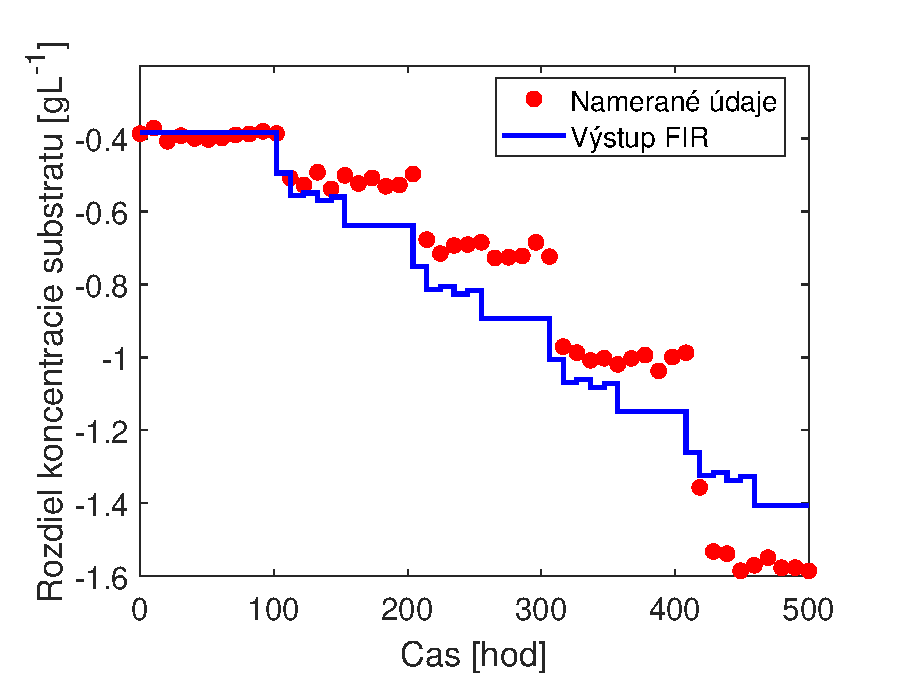
\includegraphics[width=\linewidth]{images/hybrid_multipleStep_data}
		\caption{Trénovacie dáta a výstup FIR modelu.\newline \newline}
		\label{fig:hybrid_multipleStep_data}
	\end{subfigure}
	\hfill
	\begin{subfigure}[b]{0.49\textwidth}
		\centering
		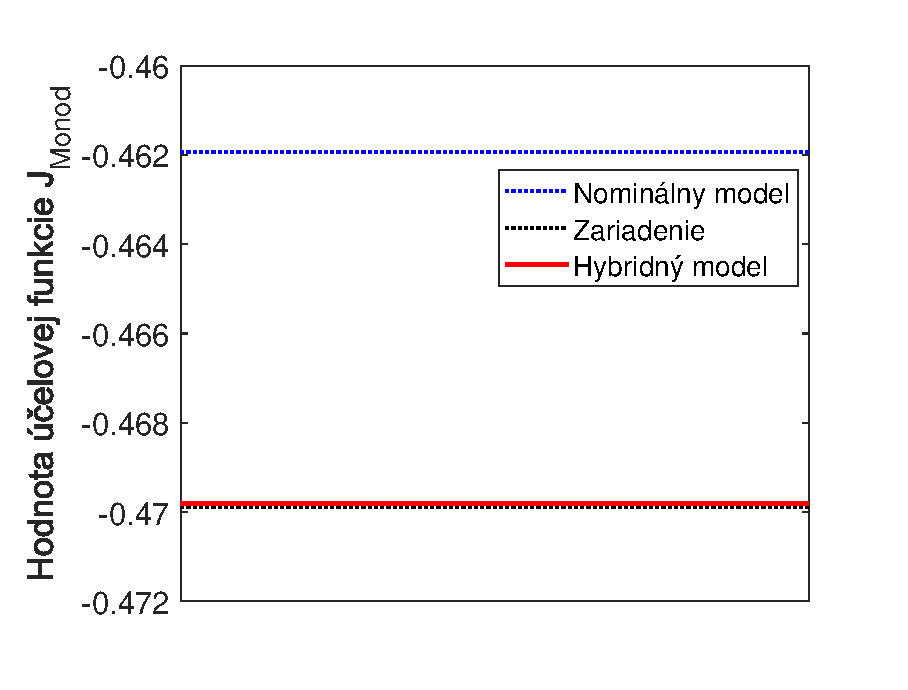
\includegraphics[width=\linewidth]{images/hybrid_multipleStep_costFun}
		\caption{Optimá hybridného modelu vyjadrené ako hodnoty účelovej funkcie Monod modelu (zariadenia).}
		\label{fig:hybrid_multipleStep_costFun}
	\end{subfigure}
	\caption{Priebeh optimalizácie zariadenia pomocou hybridného modelovania, ktorého dátová časť bola vopred natrénovaná na dátach z viacnásobnej skokovej zmeny $ D = \lbrace 0.3760, 0.3845, 0.3930, 0.4015, 0.4100 \rbrace \si{\per\hour} $.}
	\label{fig:hybrid_multipleStep_approach}
\end{figure}

Predstavme si teraz situáciu, že poznáme optimálnu rýchlosť riedenia zariadenia $ D_{P}^{\star} $. Ak spravíme skokovú zmenu z hociktorého ustáleného stavu na optimálnu hodnotu zariadenia, mali by sme získať presný rozdiel v koncentrácii substrátu, ktorý by nás z daného ustáleného stavu mal dostať do optimálneho stavu zariadenia. Pokúsme sa na týchto dátach natrénovať dátovú časť hybridného modelu a pozrime sa ako dopadne optimalizácia prevádzky zariadenia.
\begin{figure}
	\centering
	\begin{subfigure}[b]{0.49\textwidth}
		\centering
		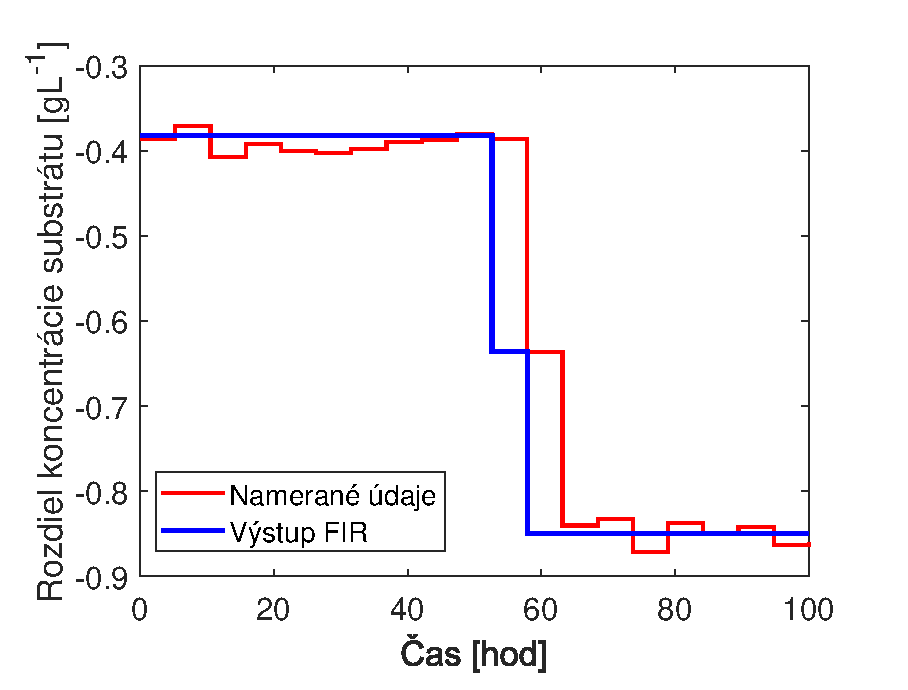
\includegraphics[width=\linewidth]{images/hybrid_optShift_data}
		\caption{Trénovacie dáta. \newline}
		\label{fig:hybrid_optShift_data}
	\end{subfigure}
	\hfill
	\begin{subfigure}[b]{0.49\textwidth}
		\centering
		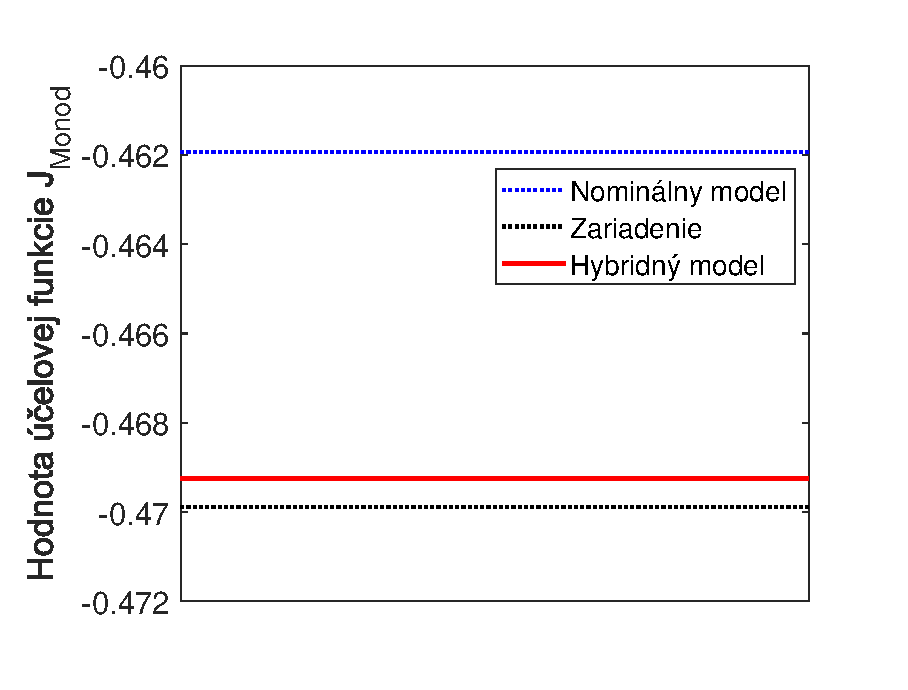
\includegraphics[width=\linewidth]{images/hybrid_optShift_costFunValues}
		\caption{Optimá vyjadrené ako hodnota účelovej funkcie Monod modelu (zariadenia).}
		\label{fig:hybrid_optShift_costFunValues}
	\end{subfigure}
	\caption{Porovnanie optím a účelových funkcií Monod (zaradenia) a hybridného modelu, ktorý bol identifikovaný na dátach zo skokovej zmeny $ D_{N}^{\star} \rightarrow D_{P}^{\star} $.}
	\label{fig:hybrid_optimum_shift}
\end{figure} 

Vykonali sme skokovú zmenu z ustáleného stavu nominálneho modelu pri rýchlosti riedenia $ D_{N}^{\star} = 0.3760\si{\per\hour} $ na hodnotu zodpovedajúcu optimálnej prevádzke zariadenia $ D_{P}^{\star} = 0.3974\si{\per\hour} $, ako uvádza Obr. \ref{fig:hybrid_optShift_data}. Skutočný rozdiel v koncentrácii ustálených stavov substrátu pri tejto rýchlosti riedenia by bol $ \Delta_{s} = -0.8448\si{\gram\per\liter} $ a FIR model identifikovaný pomocou týchto dát predikoval hodnotu rozdielu ustáleného stavu $ \Delta_{s}^{FIR} = -0.8492\si{\gram\per\liter} $. Ak máme k dispozícii presný rozdiel ustáleného stavu koncentrácie substrátu pri optimálnej rýchlosti riedenia zariadenia $ D_{P}^{\star} $, tak účelová funkcia hybridného modelu a zariadenia musia mať spoločný prienik v optime a to môžeme vidieť na Obr. \ref{fig:hybrid_and_monod_costFun_compar}. Avšak, optimum hybridného modelu nedosiahlo hodnotu optimálnej prevádzky zariadenia ako môžeme vidieť na Obr. \ref{fig:hybrid_optShift_costFunValues}. Dôvodom je, že korekcia ustáleného stavu nepresného mechanického modelu pomocou dátového modelu, štýlom aký uvádza rovnica \eqref{eq:hybrid_opt_subs} resp. \eqref{eq:hybrid_opt_bio}, neupravuje účelovú funkciu resp. jej gradient, dostatočne na to, aby sme dosiahli skutočné optimum zariadenia, ako môžeme vidieť na Obr. \ref{fig:hybrid_and_monod_costFun_compar}, ale postačuje na to, aby sme sa dostali do veľmi blízkeho okolia optima.
\begin{figure}
	\centering
	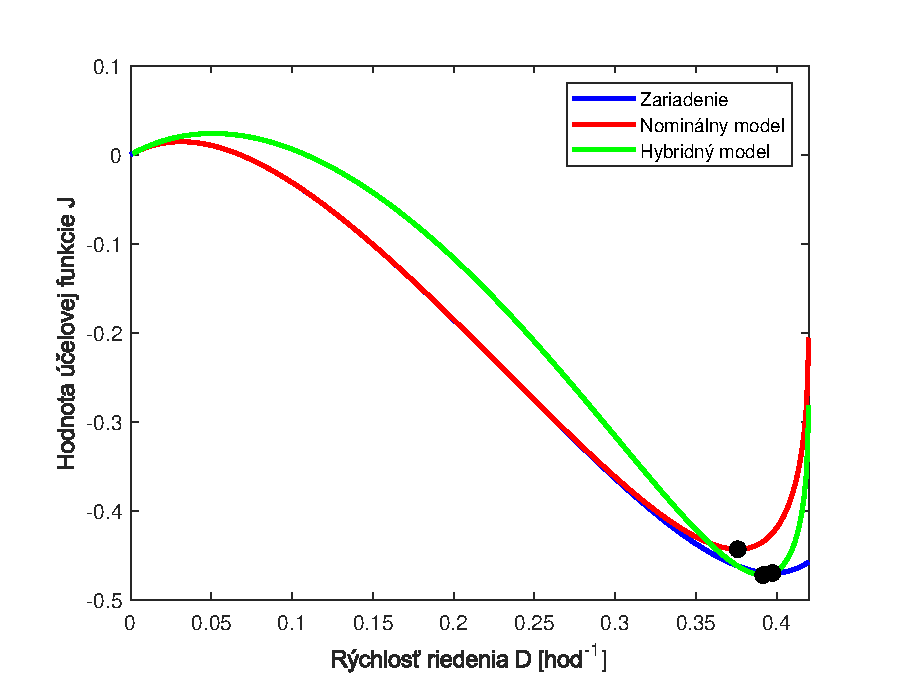
\includegraphics[width=0.7\linewidth]{images/hybrid_and_monod_costFun_compar}
	\caption{}
	\label{fig:hybrid_and_monod_costFun_compar}
\end{figure}

Mali by sme spomenúť, že hybridné modely disponujú aj predikčnými vlastnosťami, a tým pádom dokážu omnoho lepšie odhadovať výstupy zo skutočného zariadenia ako samotný nominálny model. Spravme nasledovný experiment. Nechajme schému úpravy modifikátora riešiť optimalizáciu do takej iterácie, aby nedosiahla optimum zariadenia (v našom prípade do 8. iterácie). Ná týchto dátach identifikujeme FIR model pomocou garantovaného odhadu parametrov a využijeme ho na odvodenie hybridného modelu. Trénovacie údaje sú zobrazené na Obr. \ref{fig:hybrid_dynamics_data}, kde môžeme vidieť aj výstup identifikovaného FIR modelu 3. rádu. Aby sme otestovali predikciu hybridného modelu, zvolili sme si tri rôzne rýchlosti riedenia. Dve také, ktoré boli zahrnuté v dátach na trénovanie modelu a jednu novú, optimálnu rýchlosť riedenia nášho zariadenia $ D_{P}^{\star} $, ktorá už v dátach obsiahnutá nebola. Ak testovacie dáta boli obsiahnuté v dátach na trénovanie, tak výstup z hybridného modelu dokázal veľmi presne odhadnúť skutočný výstup zo zariadenia. Na druhej strane, ak sme mu ponúkli ešte nepoznané vstupné dáta, vznikla nám odchýlka, ktorá je stále menšia ako odchýlka nominálneho modelu od zariadenia. Treba si uvedomiť, že kvalita hybridného modelu je určená kvalitou dátového modelu. To znamená, že čím lepší bude dátový model, tým lepšiu predikciu dosiahneme a vďaka garantovanej oblasti vidíme, že určité nedostatky v predikcii by sme mohli ešte zlepšiť. Na základe týchto faktov si dovolíme tvrdiť, že v oblasti riadenia by hybridné modely našli omnoho väčšie uplatnenie ako pri statickej optimalizácii.
\begin{figure}
	\centering
	\begin{subfigure}[b]{0.49\textwidth}
		\centering
		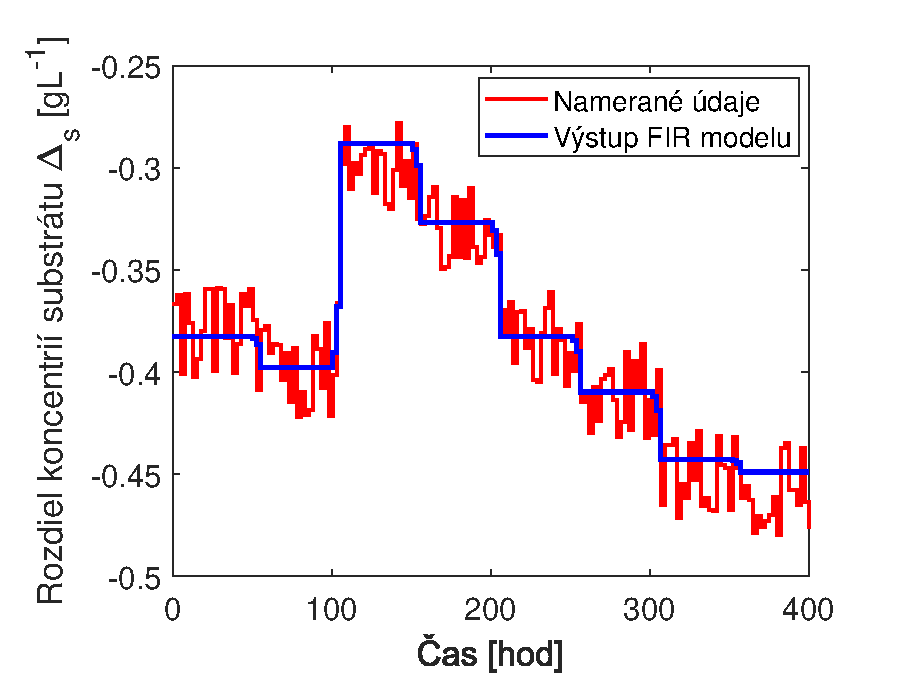
\includegraphics[width=\linewidth]{images/hybrid_dynamics_data}
		\caption{Trénovacie údaje. \newline}
		\label{fig:hybrid_dynamics_data}
	\end{subfigure}
	\hfill
	\begin{subfigure}[b]{0.49\textwidth}
		\centering
		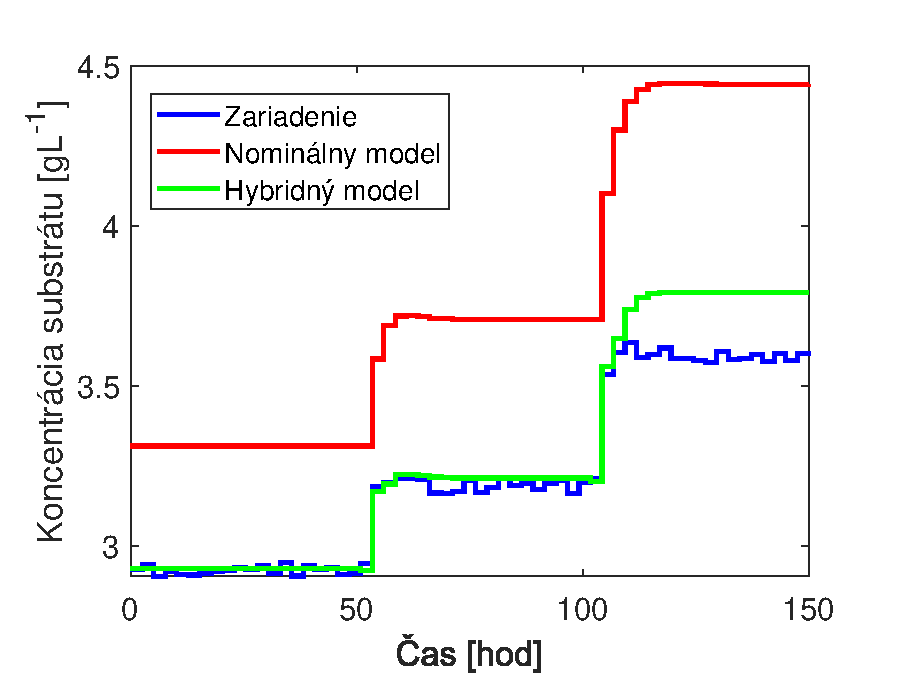
\includegraphics[width=\linewidth]{images/hybrid_dynamics_comparison}
		\caption{Porovnanie dynamiky a predikcie modelov.}
		\label{fig:hybrid_dynamics_comparison}
	\end{subfigure}
	\caption{Porovnanie predikčných schopností nominálneho a hybridného modelu, ktorý bol identifikovaný pomocou dát získaných schémou úpravy modifikátora. Testovacie vstupné údaje boli $ D = \lbrace D_{N}^{\star}, 0.385, D_{P}^{\star} \rbrace \si{\per\hour} $. Na obrázku sú znázornené priebehy koncentrácie substrátu zariadenia (tyrkysová), nominálneho modelu (ružová), minimálna (červená) a maximálna (modrá) realizácia hybridného modelu a výstup hybridného modelu identifikovaného MNŠ (zelená).}
	\label{fig:hybrid_dynamics_and_prediction}
\end{figure}

Výsledky experimentov nás priviedli k záveru, že hybridné modelovanie môže byť použité na optimalizáciu prevádzky biochemického reaktora. Uviedli sme niekoľko prístupov v rámci hybridného modelovania, ktoré sa dajú aplikovať na túto problematiku. Iteračná metóda dokázala skonvergovať v priebehu pár krokov, ale dostala sa iba do okolia optima. Ak sme dátovú časť hybridného modelu natrénovali na dopredu známych dátach, tak sme sa dostali do presného optimálneho stavu zariadenia. Netreba si však robiť ilúzie. Je veľmi pravdepodobné, že ak by sme pridali dáta zo skokových zmien pri väčších hodnotách rýchlosti riedenia, ľahko by sme optimálny stav presiahli. Ďalšou nevýhodou tohto prístupu je, že ak by sme vopred natrénovaný model zapojili do iteračnej optimalizácie, tak po niekoľkých iteráciách by sme sa vzdialili od optimálneho ustáleného stavu zariadenia. Je na to hneď niekoľko dôvodov. Jedným je, že po určitom čase nedokážeme iteračným prístupom vygenerovať informačne výdatné dáta na identifikáciu dátového modelu. A druhým je, že aj keby FIR model predikoval presný rozdiel koncentrácie substrátu zariadenia a nominálneho modelu, nikdy by sme nedosiahli skutočné optimum, ako sme ukázali na Obr. \ref{fig:hybrid_and_monod_costFun_compar}. Ak by sme chceli naše zariadenie dostať do jeho optimálneho stavu, museli by sme pozmeniť štýl, akým pristupujeme ku korekcii nominálneho modelu, napríklad tak, ako to rieši schéma úpravy modifikátora, t.j. úpravou gradientu účelovej funkcie nominálneho modelu. 
